\documentclass[12pt,a4paper,spanish]{article} 

\usepackage{graphicx} %option specific for pdfLatex compilation
\usepackage{makeidx}
\usepackage{lscape}

\usepackage[spanish]{babel}
\usepackage[utf8]{inputenc} 
\usepackage{indentfirst}

\usepackage[margin=1in]{geometry}


\begin{document}
\begin{titlepage}
\begin{center}

% Upper part of the page. The '~' is needed because \\
% only works if a paragraph has started.

\textsc{\LARGE \textbf{Universidad de Buenos Aires}}\\%[1cm]
\vfill
\textsc{\LARGE \textbf{Técnicas de Programación Concurrente I }}\\%[0.5cm]
\vfill
\textsc{\LARGE \textbf{(75.59)}}\\%[0.5cm]
\vfill
% Title
%\HRule \\[0.4cm]
\vfill
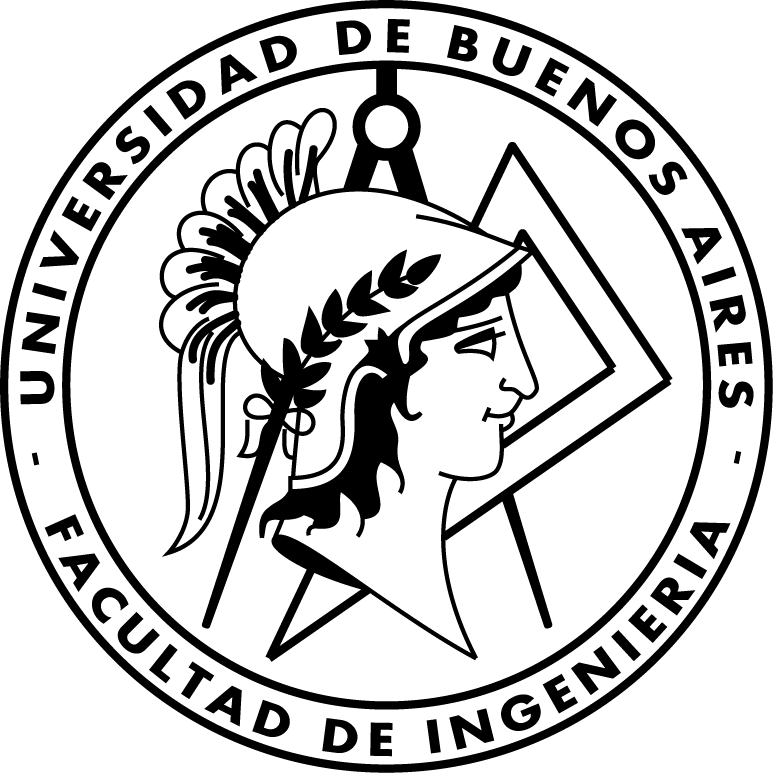
\includegraphics[scale=1.25]{./logo.png}~\\[2cm]
%\HRule \\[1.5cm]
{ \huge \bfseries Trabajo Práctico Nº 1}\\%[0.25cm]
\vfill
%{ \huge \bfseries Grupo 8}\\%[0.25cm]
%\vfill
{\Large
\begin{tabular}{|c|c|c|}
\hline
Nombre y apellido & Padrón & Mail \\
\hline
Florencia Bosch & 91867 & florb\_128@hotmail.com \\
\hline
Javier Choque & 92079 & javierchoque21@gmail.com \\
\hline
Pablo Musumeci & 92165 & pablomusumeci@yahoo.com.ar\\
\hline
\end{tabular}
}
\vfill

% Bottom of the page
{\large \today}

\end{center}
\end{titlepage}

\newpage
\tableofcontents

\section{Hipótesis}

A continuación se presentan los supuestos que consideramos a la hora de desarollar el 
trabajo práctico.


\begin{itemize}
	\item Consideramos que cuando un auto es enviado a la salida por el Jefe de Estación,
	el mismo sale del sistema de manera instantánea, sin tener que hacer una cola
	para salir de la estación.

	\item El administrador no tiene prioridad sobre los empleados al momento de consultar
	el saldo en la caja, y debido a esto, cuando desea hacerlo debe aguardar su turno para
	trabajar de manera exclusiva con la caja, al igual que cualquier empleado.

	 \item Con la finalidad de que la simulación represente una situación real, la cantidad
	 de surtidores y empleados que tiene la estación al momento de comenzar la misma debe ser 
	 mayor a 0.
\end{itemize}

\newpage

\section{Diseño}
	\subsection{Proceso Principal}

		Es el encargado de lanzar los procesos que componen la simulación, inicializar los recursos
		compartidos como semáforos y memorias compartidas.

		También se encarga de, cuando el usuario decide finalizar la simulación, enviar las señales
		apropiadas para que dichos procesos cesen el uso de los recursos. Luego, espera a la finalización
		de dichos procesos hijos, para finalizar la simulación.

	\subsection{Generador de Autos}
		
		Este proceso es el encargado de crear los autos que llegan a la estación. Para
		dicho propósito, genera autos en intervalos de tiempo especificado en el archivo de configuración. 
		Cada auto está representado por un ID y una cantidad de dinero que va a gastar en la estación.

		El Generador de Autos interactúa con el Jefe de Estación, y dicha interacción se puede
		asemejar al problema \textbf{Producer - Consumer}, debido a que el Generador produce
		los autos que el Jefe de Estación va a recibir. 

		La comunicación entre el Generador de Autos y el jefe de Estación se realiza por medio de un
		FIFO.


	\subsection{Jefe de Estación}
		Este proceso se encarga de recibir los autos nuevos que van llegando a la estación. 
		En este caso, el Jefe de Estación es el \textbf{consumer} de información.

		Una vez que logró extraer un automóvil del buffer exitosamente, debe asignarle 
		un empleado al auto recibido, en caso de que exista algun empleado disponible 
		en ese mismo instante, caso contrario, deberá redirigir el mismo hacia la salida.
		
		El jede de estación, lee un variable que se encuentra en memoria compartida, la cual
		representa el número de empleados disponibles en ese momento. Para acceder a dicha variable,
		deberá pedir acceso a un semáforo que restringe su uso de manera exclusiva.
		En el caso de exista algún empleado libre (lo cual se deduce de que el valor de dicha variable
		es mayor a cero), escribe el automóvil recibido por parte del generador en un FIFO.


	\subsection{Empleado}
	
		Este proceso representa el accionar de un empleado cuando atiende un auto. Los empleados piden acceso
		de manera exclusiva a FIFO en el que el jefe de estación escribirá los autos, de manera que no se
		atienda a un auto más de una vez por diferentes empleados. El acceso al FIFO por parte de los empleados,
		se encuentra controlado por un semáforo. 

		Una vez que un empleado recibe un auto, modifica la variable que lleva la cuenta de los empleados libres, 
		disminuyendo en uno su valor. Una vez que el empleado tiene el automóvil en su poder, se dirige hacia los
		surtidores, esperando en un semáforo que representa la cantidad de surtidores disponibles. 

		El tiempo de atención del automóvil se calcula a partir del dinero que lleva el mismo. Dicho tiempo no es
		proporcional al dinero que el automóvil dispone. Luego de la espera, libera el surtidor utilizado y se dirige
		a la caja para depositar el monto que el mismo llevaba. La caja, es implementada como una variable del tipo entero
		en memoria compartida, que debe accederse de a un proceso a la vez por medio de un semáforo.

		Cuando se finaliza la atención del automóvil, el empleado incrementa la variable que representa la cantidad
		de empleados libres, y vuelve a pedir acceso al FIFO en la espera de un nuevo cliente
	
	\subsection{Administrador}
	
	El proceso administrador tiene la facultad de consultar el valor guardado en la caja. Puede hacerlo en cualquier momento, y su consulta sobre la caja esta controlada de la misma forma que el empleado. La diferencia con el empleado es que el Administrador no espera a un auto, sino que puede consultar en cualquier momento. En nuestra implementación, 
	el administrador consulta la caja de manera periódica, siendo configurable el período de espera entre cada consulta.

\subsection{Casos de uso}

\begin{itemize}
	\item Inicar simulación: El actor que dispara este caso de uso es el usuario
	que desea iniciar la simulación. Para iniciar el programa se debe ejecutar el
	proceso \texttt{procesoPrincipal}, el cual se encarga de
	lanzar a los otros procesos involucrados en el funcionamiento de la simulación.

	Es necesario que la ejecución del proceso principal se realize con los parámetros
	que indican la cantidad de empleados (por medio de la expresión \texttt{-e} o \texttt{--empleados})
	y la cantidad de surtidores (\texttt{-s} o \texttt{--surtidores})que que tendrá la
	estación de servicio.

	Ejemplo:

	\texttt{./procesoPrincipal -e 5 -s 7}

	\item Finalizar la simulación: El proceso principal se quedará esperando por el 
	ingreso de un caracter cualquiera, como orden para finalizar todos los procesos
	que componen la simulación.

\end{itemize}


	\section{Diagrama esquemático de interacciones}
	
	Ver figura \ref{diagrama}

\begin{figure}
\label{diagrama}
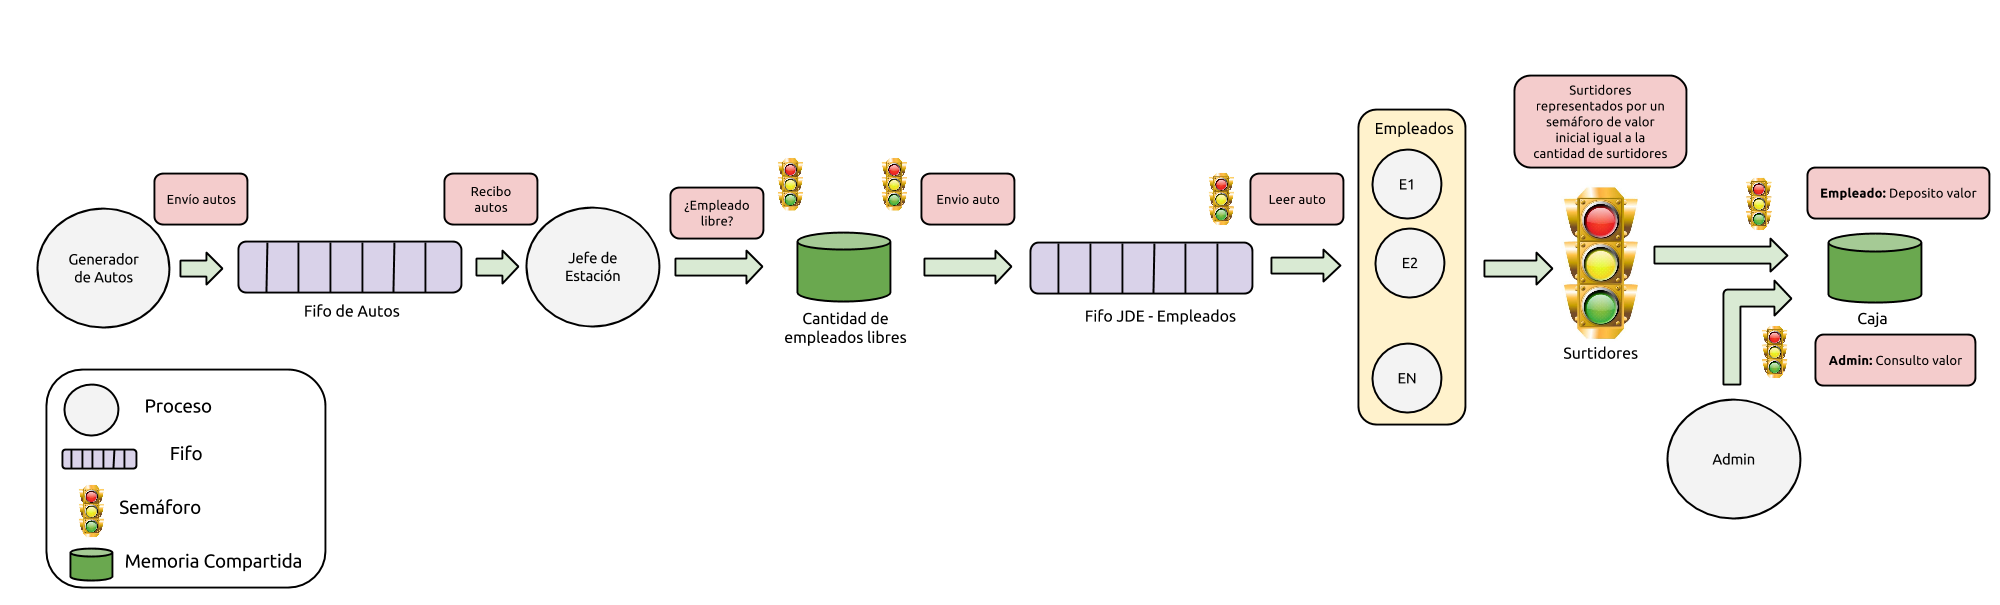
\includegraphics[angle=90, scale = 0.34]{esquema.png}
\centering
\caption{Diagrama esquemático de interacciones}
\end{figure}

\newpage
	\section{Datos compartidos entre procesos}
	
	\begin{itemize}
	
	\item Generador de Autos - Jefe de Estación:
		\begin{itemize}
			\item Fifo \texttt{files/generador.jde} para envío de los autos
		\end{itemize}
	
	\item Jefe de Estación - Empleado:
	\begin{itemize}
		\item Fifo \texttt{files/jde.empleado} para envío de los autos
		\item Memoria compartida con la cantidad de empleados disponibles
		\item Semáforo para controlar acceso a la memoria compartida.
		\item Semáforo para controlar acceso al Fifo, por parte del empleado (lector).
	\end{itemize}

	\item Empleado (surtidores):
	\begin{itemize}
		\item Semáforo \texttt{files/semaforo.surtidores} que representa la 
		cantidad de surtidores libres, y controla el acceso a los mismos.
	\end{itemize}

	\item Empleado (caja):
	\begin{itemize}
		\item Memoria compartida que representa la caja
		\item Semáforo que controla el acceso a la caja
	\end{itemize}

	\item Administrador (caja):
	\begin{itemize}
		\item Memoria compartida que representa la caja
		\item Semáforo que controla el acceso a la caja
	\end{itemize}

	\end{itemize}
	\newpage
	\section{Diagrama de estados del proceso Jefe De Estación}

	\begin{figure}[h]
	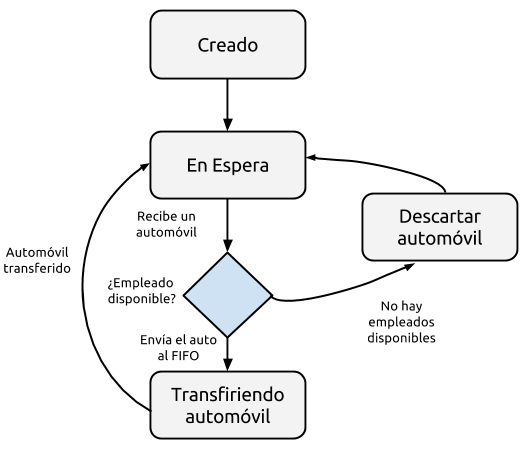
\includegraphics[scale=0.75]{FSM_JDE.png}
	\centering
	% https://docs.google.com/drawings/d/1fSqCpKnnYxksGUfpufRSJbsfxkYRRuSEGUDkyJf5Sf0/edit?usp=sharing
	\caption{FSM del Jefe de Estación}
	\end{figure}

	\newpage
	\section{Diagramas de clases}
	\subsection{Generador de automóviles y Jefe de estación}
	\begin{figure}[h]
	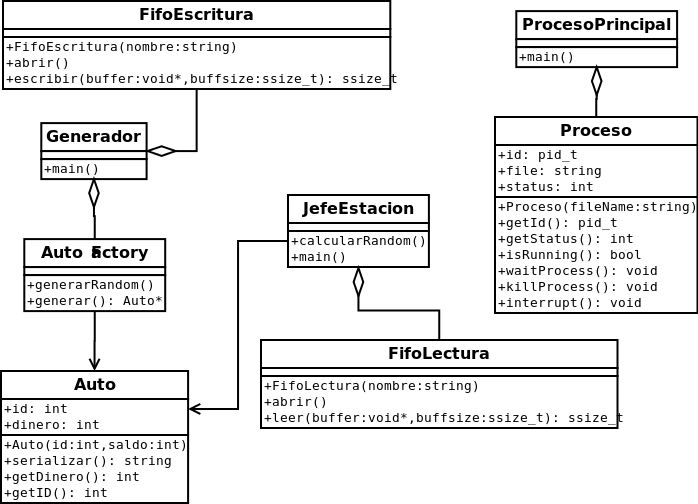
\includegraphics[scale=0.60, angle=90]{GeneradorJde.png}
	\centering
	\end{figure}

	\newpage		
	\subsection{Jefe de estación y empleado}
	\begin{figure}[h]
	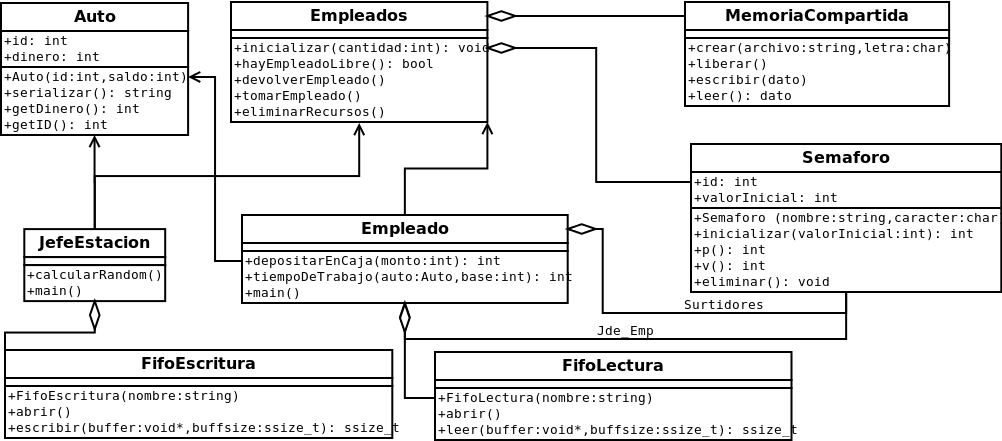
\includegraphics[scale=0.50, angle=90]{JDE_Empleado.png}
	\centering
	\end{figure}

	\newpage	
	\subsection{Empleados, administrador y acceso a la caja}
	\begin{figure}[h]
	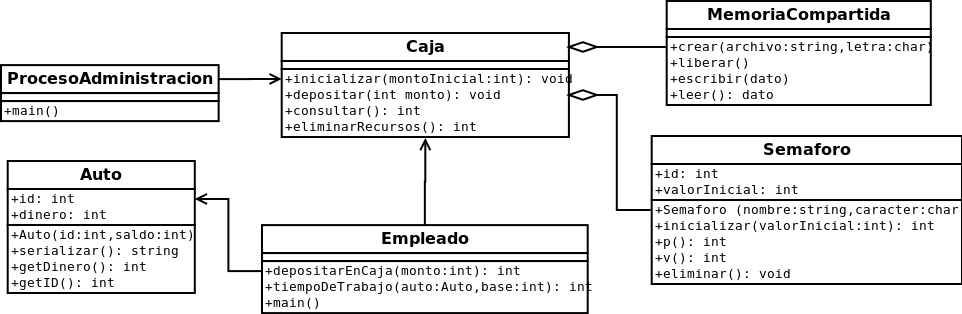
\includegraphics[scale=0.50, angle=90]{AccesoCaja.png}
	\centering
	\end{figure}

\end{document}
